\section{Networks}
\label{sec:xbrl_networks}

Up to this point, all concepts in the XBRL taxonomy are treated as independent entities.
The whole filing can be viewed as an unordered set of facts with no relation between them.
However, in reality, concepts are not independent of each other.
Instead, concepts are often related to each other in some way.

For example, the concepts \texttt{Assets} and \texttt{Liabilities} are related to each other in the sense that they are both part of the concept \texttt{Balance Sheet}.
Furthermore, the concept \texttt{Assets} can be further divided into the concepts \texttt{Current Assets} and \texttt{Non-Current Assets}.
The afforementioned relations can be visualized using a directed graph, as shown in figure \ref{fig:example_visualization_network_xbrl}.

\begin{figure}[H]
    \caption{Example of a relations between concepts in XBRL}
    \label{fig:example_visualization_network_xbrl}
    \dirtree{%
        .1 Balance Sheet.
        .2 Assets.
        .3 Current Assets.
        .3 Non-Current Assets.
        .2 Liabilities.
    }
\end{figure}

A reader with a basic understanding of mathematics will recognize that the above example is a directed acyclic graph (DAG).
More specifically, the above example is a tree.
Graphs are commonly used to represent relations between entities.
In the context of XBRL, graphs are used to represent all kinds of relations between concepts, facts, and other elements of an XBRL filing.
From now on, I will refer to graphs that represent relations between concepts as \texttt{networks}.

XBRL commonly refers uses the term \texttt{Extended Link} or \texttt{Link} to refer to networks or parts of networks.
I will use the term \texttt{network} throughout this thesis, since it is more intuitive and less ambiguous.
When I refer to a \texttt{link}, I am referring to something specific in the XBRL specification.
When I refer to a \texttt{network}, I am referring to the general concept of a network.

XBRL groups multiple links together into so called \texttt{linkbases}.
From a semantic perspective, linkbases do not have any meaning.
From a technical perspective, linkbases are just XML elements that have children that are links. 

\subsection{Types of Networks}

The XBRL 2.1 specification defines 6 built in types of networks\cite{xbrl21_terminology}\footnote[1]{The XBRL 2.1 specification is inconsistent about \texttt{link:footNotelink}. Section 1.4 does not list it as a standard extended link, section 3.5.2.4 does. I will assume that it is a standard extended link.}:

\begin{itemize}
    \item \texttt{link:presentationLink}: A network that represents the hierarchy of concepts in a report. An example of this can be seen in figure \ref{fig:example_visualization_network_xbrl}.
    \item \texttt{link:calculationLink}: A network that represents how concepts are calculated from other concepts. 
    For example, in figure \ref{fig:example_visualization_network_xbrl}, the concept \texttt{Assets} is calculated as the sum of the concepts "Current Assets" and "Non-Current Assets".
    \item \texttt{link:definitionLink}: A network that represents the relations between concepts and their definitions. 
    For example, there might be a concept \texttt{TotalAssets} that has the same semantic meaning as the concept \texttt{Assets}. 
    A definition network would represent that the two concepts are aliases of each other.
    \item \texttt{link:labelLink}: A network that associates report elements with human-readable labels.
    \item \texttt{link:referenceLink}: A network that links report elements to external resources. 
    For example, the concept \texttt{Total Shareholder Return Amount} might have an official definition in the SEC's Code of Federal Regulations (CFR).
    The reference network would link the concept to the subparagraph \texttt{17 CFR 229.402(v)(2)(iv)}\cite{cfr_total_shareholder_return_amount}.
    \item \texttt{link:footnoteLink}: A network that links report elements, facts and other elements to footnotes.
\end{itemize}

XBRL refers to these built in networks as \texttt{standard extended links}. 
If needed, XBRL allows users to define their own networks, which are referred to as \texttt{custom extended links}\cite{xbrl21_terminology}.

Technically speaking, XBRL does allow networks in XBRL to contain both directed and undirected cycles.
However, in practice, networks in XBRL are almost always directed acyclic graphs (DAGs).

In the subsequent sections, I will describe how networks are implemented in XBRL on a conceptual level. 

TODO: add a simple explanation of labels since I use them throughout this chapter

\subsection{presentationLink}

The \texttt{link:presentationLink} network is used to represent the hierarchy of concepts in a report.
I will describe presentationLinks in more detail compared to the other networks, since the other network types are implemented in a similar way.

XBRL implements all its networks as a set of directed edges called \texttt{arcs}.
Each arc has a source and a target. Duplicate arcs are not allowed.

Taking the example from figure \ref{fig:example_visualization_network_xbrl}, the presentationLink network would be represented as the following edge list:

% dont use the minted package
\begin{figure}[H]
    \caption{Example of a presentationLink network in edge list format}
    \label{fig:example_visualization_network_xbrl_edge_list}
    \begin{verbatim}
        Balance Sheet -> Assets
        Assets -> Current Assets
        Assets -> Non-Current Assets
        Balance Sheet -> Liabilities
    \end{verbatim}
\end{figure}

Each arc in the example \ref{fig:example_visualization_network_xbrl_edge_list} is represented as a \texttt{link:presentationArc} element in XBRL.
Besides presentationArcs, presentationLinks contain so called "locators" \texttt{link:loc} that represent the nodes in the network.
In case of a presentaton network, the locators are references to the concepts in the XBRL taxonomy. 
In other networks, locators can be references to other elements, such as facts.

In case of the XML syntax, the first \texttt{link:presentationArc} "Balance Sheet -> Assets" would be represented as follows:

\begin{figure}[H]
    \begin{lstlisting}[language=XML]
        <link:loc 
            xlink:type="locator" 
            xlink:href="file_1.xsd#BalanceSheet"
            xlink:label="BalanceSheet_loc"
        />
        <link:loc 
            xlink:type="locator" 
            xlink:href="file_1.xsd#Assets"
            xlink:label="Assets_loc"
        />
        <link:presentationArc 
            xlink:type="arc" 
            xlink:arcrole="http://www.xbrl.org/2003/arcrole/parent-child" 
            xlink:from="BalanceSheet_loc" 
            xlink:to="Assets_loc"
            order="1"
        />
    \end{lstlisting}
    \caption{Example of a presentationArc in XML syntax}
    \label{fig:example_presentation_arc_xml}
\end{figure}

The \texttt{xlink:from} attribute of the \texttt{link:presentationArc} element references the \texttt{xlink:label} attribute of the \texttt{link:loc} element that represents the source of the arc.
The same applies to the \texttt{xlink:to} attribute of the \texttt{link:presentationArc} element.

Both locators contain a \texttt{xlink:href} attribute that references the concept in the XBRL taxonomy that the locator represents.
This reference can even point to a different file, as shown in figure \ref{fig:example_presentation_arc_xml}.

The \texttt{xlink:type} on the elements helps the XML parser to determine the type of the element.
Note that the XML tag \texttt{link:presentationArc} already hints at the fact that this element is a type of arc.
However, the \texttt{xlink:type} attribute is still required and provides parsers with a more reliable way to determine if an element is an arc, a locator, or something else. 

The \texttt{order} attribute of the \texttt{link:presentationArc} element specifies in which order the children of the source of the arc should be displayed.

\label{sec:arcrole}
Finally, the \texttt{xlink:arcrole} attribute of the \texttt{link:presentationArc} element specifies the kind of relation between the source and the target of the arc.
In case of a presentationLink, the \texttt{xlink:arcrole} attribute is always set to \texttt{parent-child}.
For different networks, the \texttt{xlink:arcrole} attribute can be set to different values.
It can even be set to different values for different arcs in the same network.

XBRL packages the set of arcs and locators into a \texttt{link:presentationLink} element.
This element contains a \texttt{xlink:role} attribute that specifies the role of the presentationLink.
Roles are a more advanced concept that I will introduce in section \ref{sec:roles}.
For now, think of the \texttt{link:presentationLink} element as a container for the arcs and locators.

\subsection{Motivation for Report Elements}
\label{sec:report_elements_motivation}

Up to this point, I have only described how presentation networks are implemented in XBRL.
I also mentioned that presentation networks indroduce a hierarchy of concepts, but this is not entirely true.

I have introduced concepts as the "what"-part of a fact. 
For example, if the company Foo reports a revenue of 1000 USD in 2019, the concept \texttt{Revenue} is the "what"-part of the fact.

However, if we look at the presentation network in figure \ref{fig:example_visualization_network_xbrl}, not all of the elements in the network can have a fact associated with them.
For example, the concept \texttt{BalanceSheet} cannot have a fact associated with it.
In XBRL, concepts that can not have a fact associated with them are called \texttt{Abstract}.

The Open Information Model (OIM) combines abstracts and concepts using the term \texttt{report element}.
Report elements are, as the name suggests, elements that can appear in a report.
Some of these report elements are used for facts, namely the concepts.
Others are used to represent the structure of the report, namely the abstracts.
There are six types of report elements in total\cite{oim}. 
I will introduce them as they come up in the subsequent sections.

With the introduction of report elements, our notion of a presentation network changes slightly.
Instead of introducing a hierarchy of concepts, presentation networks introduce a hierarchy of report elements.
However, our notion of a fact stays the same.
A fact is still requires a concept, not a report element.

\subsection{calculationLink}

The \texttt{link:calculationLink} network is used to represent how concepts are calculated from other concepts.
More specifically, it is used to represent how a concept is the sum of other concepts.
Under the hood, calculationLinks are implemented in the same way as presentationLinks, but there are a few differences in the semantics.

\begin{enumerate}
    \item The arcs now have the tag \texttt{link:calculationArc} instead of \texttt{link:presentationArc}.
    \item The link now has the tag \texttt{link:calculationLink} instead of \texttt{link:presentationLink}.
    \item The \texttt{xlink:arcrole} attribute of the \texttt{link:calculationArc} element is set to \texttt{summation-item}.
    \item The \texttt{link:calculationArc} element has an additional attribute called \texttt{weight}.
    \item All locators in the link are references to concepts, not just report elements.
\end{enumerate}

Most of these differences are self-explanatory and do not have any semantic implications.
However, the last two differences are worth explaining in more detail.

The main motivation behind calculation networks is so that XBRL processors can either calculate the value of a concept or check if the value of a concept is computed correctly and consistently.
In the case of our XBRL processor Brel, the main focus is on the latter. 
Chapter 6.4 of "The XBRL Book" \cite{fourny2023xbrl} describes the different consistency checks in more detail.

Concepts within a calculation network are computed as a weighted sum of their children.
The \texttt{weight} attribute of the \texttt{link:calculationArc} element specifies the weight of the child in the sum.
Additionally, facts can only be associated with concepts, not just any report element.
Therefore, all locators in a calculation network are references to concepts.

In the section on concepts\ref{sec:concepts}, I have introduced the \texttt{balance} aspect of a concept.
It specifies if the concept is a debit or a credit.
The XBRL 2.1 specification enforces some constraints on the \texttt{balance} aspect of concepts in combination with the \texttt{weight} attribute of the \texttt{link:calculationArc} element \cite{xbrl21_concept}.
If one concept has a \texttt{balance} of \texttt{debit} and another concept has a \texttt{balance} of \texttt{credit}, then their connecting arc must have a negative \texttt{weight}.
If both concepts have the same \texttt{balance}, then their connecting arc must have a positive \texttt{weight}.

% small table describing the balance and weight constraints
\begin{figure}[H]
    \label{fig:balance_weight_constraints}
    \centering
    \begin{tabular}{|l|l|l|}
        \hline
        \textbf{Concept 1} & \textbf{Concept 2} & \textbf{Connecting edge weight} \\ \hline
        Debit              & Credit             & $\leq 0$        \\ \hline
        Credit             & Debit              & $\leq 0$        \\ \hline
        Debit              & Debit              & $\geq 0$        \\ \hline
        Credit             & Credit             & $\geq 0$        \\ \hline
    \end{tabular}
    \caption{Balance and weight constraints in calculation networks}
\end{figure}

A network that is consistent with the balance and weight constraints is called a \texttt{balance consistent network}.\cite{fourny2023xbrl}

Balance consistency is not the only kind of consistency that calculation networks can be checked for.
Another kind of consistency is \texttt{roll-up consistency} which comes in two flavors: \texttt{simple roll-up consistency} and \texttt{nested roll-up consistency}. 

Simple roll-up is roll-up consistency without any nested concepts. 
So the calculation network can only have a depth of 1.

Nested roll-up consistency is roll-up consistency with nested concepts.
So the calculation network can have a depth of more than 1.

\texttt{Roll-up consistency} requires a calculation network as well as a presentation network and checks if the structure of the two networks is consistent.
For example, if the calculation network contains the arc \texttt{Assets -> Savings Accounts}, 
then the presentation network must also contain the arc \texttt{Assets [Abstract] -> Savings Accounts}.

Remember that calculation networks can only contain concepts, not abstracts. 
So the report element \texttt{Assets} in the calculation network and the report element \texttt{Assets [Abstract]} in the presentation network are not the same.
But how does XBRL know that they are related?

The answer is that the two report elements are related by the presentation network.
It contains the arc \texttt{Assets [Abstract] -> Assets}.

Let us visualize this example in figure \ref{fig:example_roll_up_consistency}, 
which shows the calculation network and the presentation network side by side.
The example is expanded a bit and also contains the concepts \texttt{UBS Savings Account}, \texttt{Raiffeisen Savings Account} and \texttt{Liabilities}.

\begin{figure}[H]
    \caption{Example of nested roll-up consistency}
    \label{fig:example_roll_up_consistency}
    % draw the calculation- and presentation network side by side
    \begin{minipage}{0.8\textwidth}
        \dirtree{%
            .1 Assets (weight: 1).
            .2 Savings Accounts (weight: 1).
            .3 UBS Savings Account (weight: 1).
            .3 Raiffeisen Savings Account (weight: 1).
            .2 Liabilities (weight: -1).
        }
        \caption{Calculation network}
    \end{minipage}
    \begin{minipage}{0.8\textwidth}
        \dirtree{%
            .1 Assets [Abstract].
            .2 Savings Accounts [Abstract].
            .3 UBS Savings Account.
            .3 Raiffeisen Savings Account.
            .3 Savings Accounts.
            .2 Assets.
            .2 Liabilities.
        }
        \caption{Presentation network}
    \end{minipage}
\end{figure}

The presentation network in figure \ref{fig:example_roll_up_consistency} is roll-up consistent with the calculation network.
It contains the two abstracts \texttt{Assets [Abstract]} and \texttt{Savings Accounts [Abstract]}, 
which are not present in the calculation network. 
They take the role of the concepts \texttt{Assets} and \texttt{Savings Accounts} in the calculation network.

Besides roll-up and balance consistency, there is a third kind of consistency. 
XBRL does not have a name for it, but I will refer to it as \texttt{aggregation consistency}.
It checks if in a calculation network, for each concept, the child concepts add up to their parent concept.
Going back to our example in figure \ref{fig:example_roll_up_consistency},
the values of the UBS Savings Account and the Raiffeisen Savings Account should add up to the value of the Savings Accounts concept.
Aggregation consistency uses weighted sums to add up the values of the child concepts, 
where the weight of a child concept is the weight of the connecting arc.

To check for aggregation consistency, we need to know the values of the facts that are associated with the concepts.
So aggregation consistency checks a list of facts against a calculation network.

Aggregation consistency is best explained using an example.
Consider the following list of facts for the calculation network in figure \ref{fig:example_roll_up_consistency}:

% \begin{figure}[H]
%     \caption{List of facts for the calculation network in figure \ref{fig:example_roll_up_consistency}}
%     \label{fig:example_facts}
%     \begin{tabular}{|r|r|r|r|l|}
%         \hline
%         \textbf{Concept} & \textbf{Entity} & \textbf{Period} & \textbf{Unit} & \textbf{Value} \\ \hline
%         UBS Savings Account & Alice & 2019 & USD & 1000 \\ \hline
%         Raiffeisen Savings Account & Alice & 2019 & USD & 2000 \\ \hline
%         Savings Accounts & Alice & 2019 & USD & 3000 \\ \hline
%         Liability & Alice & 2019 & USD & 500 \\ \hline
%         Assets & Alice & 2019 & USD & 2500 \\ \hline
%         UBs Savings Account & Alice & 2020 & USD & 2000 \\ \hline
%         Raiffeisen Savings Account & Alice & 2020 & USD & 3000 \\ \hline
%         Savings Accounts & Alice & 2020 & USD & 5000 \\ \hline
%         Liability & Alice & 2020 & USD & 1000 \\ \hline
%         Assets & Alice & 2020 & USD & 3999 \\ \hline
%     \end{tabular}
% \end{figure}

\begin{figure}[H]
    \caption{Alice's savings accounts and liabilities in CHF}
    \label{fig:example_facts_aggregation_consistency}
    \centering 
    \begin{tabular}{|r|r|r|}
        \hline
        \textbf{Concept} & \textbf{2022} & \textbf{2023} \\ \hline
        UBS Savings Account & 1000 & 1000 \\ \hline
        Raiffeisen Savings Account & 2000 & 3000 \\ \hline
        Savings Accounts & 3000 & 4000 \\ \hline
        Liability & 500 & 500 \\ \hline
        Assets & 2500 & 3499 \\ \hline
    \end{tabular}
\end{figure}

The list of facts in figure \ref{fig:example_facts_aggregation_consistency} can be checked for aggregation consistency against the calculation network in figure \ref{fig:example_roll_up_consistency}.
As you can see, there are two facts reported against each concept, one for 2022 and one for 2023.

If there are multiple facts reported against a concept, then we iterate over them and "pin" all aspects except for the concept.
Next, we go to the list of all facts and filter out all facts that have the same pinned aspects.
Finally, we check for aggregation consistency using the filtered list of facts and the calculation network.

In our example, we would first check all facts for 2022, then all facts for 2023.
The list of facts is aggregation consistent for the year 2022, since the values of the UBS Savings Account and the Raiffeisen Savings Account add up to the value of the Savings Accounts concept.
Also, the value of the Savings Accounts minus the value of the Liabilities concept adds up to the value of the Assets concept.

However, the list of facts is not aggregation consistent for the year 2023.
The reason being that the value of the Savings Accounts minus the value of the Liabilities concept does not result in the value of the Assets concept.

\subsection{definitionLink}

TODO

\subsection{labelLink}
\label{sec:labelLink}

The \texttt{link:labelLink} network is used to associate report elements with human-readable labels.
Thus far, we referred to report elements using their QName.
Obviously, if you open an XBRL report in a viewer such as Arelle, you do not see any QNames for the concepts, abstracts, etc.
Instead, you see human-readable labels.

The following figure shows an example of the condensed consolidated statement of income of the Coca Cola Company\cite{ko2019q2} of Q2 2019 as displayed in Arelle\cite{arelle}.

\begin{figure}[H]
    \centering
    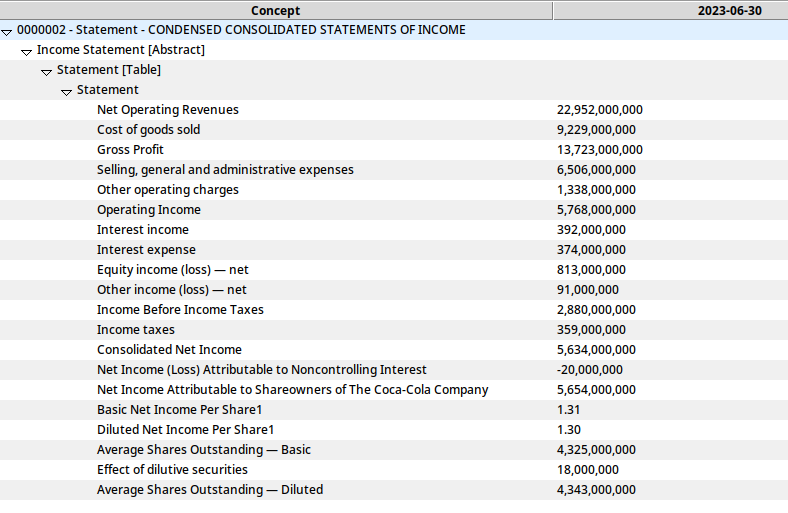
\includegraphics[width=\textwidth]{images/coca_cola_2019_q2.png}
    \caption{Statement of income of the Coca Cola Company of Q2 2019}
    \label{fig:coca_cola_2019_q2}
\end{figure}

Let us take a closer look at the first concept of the statement of income: Revenue.
Even though the concept for the revenue is \texttt{us-gaap:Revenues}, Arelle displays it as "Net Operating Revenues".

Arelle achieves this by using the \texttt{link:labelLink} network that is part of the XBRL report. 
LabelLinks are another type of extended link that associates report elements with human-readable labels.
They are implemented in the same way as presentationLinks and calculationLinks, but this time they not only contain arcs and locators, but also \texttt{link:label} elements.

From a semantic perspective, labels are different from report elements such as concepts and abstracts.
Instead, they are a kind of \texttt{resource}.
Resources are essentially metadata about report elements, facts, and other elements of an XBRL report.

The approach that XBRL takes to labels and other resources is quite interesting.
Going back to our example in figure \ref{fig:coca_cola_2019_q2}, the definition of the concept \texttt{us-gaap:Revenues} happens independently from any labels that are associated with it.
The labels are later associated with the concept using the \texttt{link:labelLink} network.
In fact, each report element can have multiple labels associated with it.
These labels can be in different languages or can have different roles.
Roles are a covered later in this chapter.
We have already seen the \texttt{xlink:arcrole} attribute in the \texttt{link:presentationArc} \ref{sec:arcrole}.
The role of a label works in a similar way.

In terms of the XML syntax, the \texttt{link:labelLink} network is implemented in the same way as the \texttt{link:presentationLink} network.
The only addition is the \texttt{link:label} element, which is used to represent a label.
It contains a few pieces of information:

\begin{enumerate}
    \item The \texttt{xlink:label} attribute, which is used to reference the arc that the label is associated with.
    This must not be confused with the text of the label.
    Think of it as a unique identifier for the label.
    \item The \texttt{xlink:role} attribute, which specifies the role of the label. More on this later.
    \item The \texttt{xml:lang} attribute, which specifies the language of the label.
    \item The \texttt{xlink:type} which is always set to \texttt{resource}.
    \item The actual label text. This is the human-readable label that is displayed in Arelle.
\end{enumerate}

For example, for the label "Net Operating Revenues" \ref{fig:coca_cola_2019_q2}, the following XML segment would be used:

\begin{figure}[H]
    \begin{lstlisting}[language=XML]
        <link:label 
          id="1234" 
          xlink:label="lab_us-gaap_Revenues" 
          xlink:role="http://www.xbrl.org/2003/role/terseLabel" 
          xlink:type="resource" 
          xml:lang="en-US">
            Net Operating Revenues
        </link:label>

    \end{lstlisting}
    \caption{Example of a label in XML syntax}
    \label{fig:example_label_xml}
\end{figure}

Note that we have omitted both the connecting arc and the locator in this example.
Both arcs and locators work in the same way as in the \texttt{link:presentationLink} network.

% % Arc and locator of the example above
% <link:loc 
%     xlink:type="locator" 
%     xlink:label="loc_us-gaap_Revenues" 
%     xlink:href="us-gaap-2023.xsd#us-gaap_Revenues"/>
% <link:labelArc 
%     xlink:arcrole="http://www.xbrl.org/2003/arcrole/concept-label" 
%     xlink:from="loc_us-gaap_Revenues" 
%     xlink:to="lab_us-gaap_Revenues" 
%     xlink:type="arc" 
%     order="1"/>

The label in figure \ref{fig:example_label_xml} has the role \texttt{http://www.xbrl.org/2003/role/terseLabel}.
This role is used to indicate that the label is a short, human-readable label.
XBRL defines a few other roles of which the most important ones are:

\begin{figure}[H]
    \begin{tabular}{|l|l|}
        \hline
        \textbf{Role} & \textbf{Description} \\ \hline
        \texttt{http://www.xbrl.org/2003/role/label} & The default label role. \\ \hline
        \texttt{http://www.xbrl.org/2003/role/terseLabel} & A short, human-readable label. \\ \hline
        \texttt{http://www.xbrl.org/2003/role/verboseLabel} & A long, human-readable label. \\ \hline
        \texttt{http://www.xbrl.org/2003/role/positiveLabel} & A label for positive values. \\ \hline
        \texttt{http://www.xbrl.org/2003/role/negativeLabel} & A label for negative values. \\ \hline
        \texttt{http://www.xbrl.org/2003/role/zeroLabel} & A label for zero values. \\ \hline
        \texttt{http://www.xbrl.org/2003/role/documentation} & A label for documentation. \\ \hline
    \end{tabular}
    \caption{Important label roles}
    \label{fig:important_label_roles}
\end{figure}

Note that the list of label roles is not exhaustive.
There are many more label roles that are used in practice. 
Users can even define their own label roles.
For a complete list of standard label roles, refer to the XBRL 2.1 specification\cite{xbrl21_label_roles}.

\subsection{referenceLink}

The \texttt{link:referenceLink} network is used to link report elements to external resources.
For example, the concept \texttt{us-gaap:Revenues} might have an official definition in the SEC's Code of Federal Regulations (CFR).
The reference establishes a link between the concept and external resource such as the CFR.
Intuitively, think of the reference as a citation in a scientific paper.

Structurally, referenceLinks are implemented in the same way as LabelLinks - they contain arcs, locators, and resources.
The only difference is that the resources are references to external resources, not labels.
Whereas labels are mostly just text, references are take the form of dictionaries.

The following figure shows an example of a reference in the XML syntax with an accompanying locator and arc.

\begin{figure}[H]
    \begin{lstlisting}[language=XML]
        <link:loc 
            xlink:type="locator" 
            xlink:href="#ecd_CoSelectedMeasureName" 
            xlink:label="CoSelectedMeasureName"
        />
        
        <link:reference xlink:type="resource" xlink:label="SECRegulationS-K229402v2vi" xlink:role="http://www.xbrl.org/2003/role/presentationRef">
            <ref:Publisher>SEC</ref:Publisher>
            <ref:Name>Regulation S-K</ref:Name>
            <ref:Number>229</ref:Number>
            <ref:Section>402</ref:Section>
            <ref:Subsection>v</ref:Subsection>
            <ref:Paragraph>2</ref:Paragraph>
            <ref:Subparagraph>vi</ref:Subparagraph>
        </link:reference>
        
        <link:referenceArc 
            xlink:type="arc" 
            xlink:arcrole="http://www.xbrl.org/2003/arcrole/concept-reference" 
            xlink:from="CoSelectedMeasureName" 
            xlink:to="SECRegulationS-K229402v2vi" 
            priority="10"
        />
    \end{lstlisting}
    \caption{Example of a reference for the concept \texttt{edc:CoSelectedMeasureName}}
    \label{fig:example_reference_xml}
\end{figure}

We are already familiar with the \texttt{link:loc} and \texttt{link:referenceArc} elements. 
The only notworthy change to the \texttt{link:referenceArc} element is the \texttt{xlink:arcrole} attribute, which is set to \texttt{concept-reference}.

However, our main focus is on the \texttt{link:reference} element, more specifically, its children.
The children of the \texttt{link:reference} element form a dictionary that describes the external resource that the reference points to.

In the example \ref{fig:example_reference_xml}, the reference points to a subparagraph of the SEC's Code of Federal Regulations (CFR).
References can point to any kind of external resource, not just the CFR.
They can point to other XBRL reports, PDFs, websites, etc.

Usually, an XBRL report contains only one referenceLink, 
which is used to link the concepts in the report to the concepts to the underlying code of regulations.

\subsection{footnoteLink}

The \texttt{link:footnoteLink}, just like the \texttt{link:referenceLink} and the \texttt{link:labelLink}, is used to associate report elements with resources.
One difference is that the resources are footnotes, not labels or references, which is a surface level difference.
The other difference is that the locators in the footnoteLink can also reference facts, not just report elements.
Other than that, footnoteLinks are implemented in the same way as the other networks.